\documentclass[simplex.tex]{subfiles}
% NO NEED TO INPUT PREAMBLES HERE
% packages are inherited; you can compile this on its own

\onlyinsubfile{
\title{NeuroData SIMPLEX Report: Subfile}
}

\begin{document}
\onlyinsubfile{
\maketitle
\thispagestyle{empty}

The following report documents the progress made by the labs of Randal~Burns and Joshua~T.~Vogelstein at Johns Hopkins University towards goals set by the DARPA SIMPLEX grant.

%%%% Table of Contents
\tableofcontents

%%%% Publications
\bibliographystyle{IEEEtran}
\begin{spacing}{0.5}
\section*{Publications, Presentations, and Talks}
%\vspace{-20pt}
\nocite{*}
{\footnotesize	\bibliography{simplex}}
\end{spacing}
%%%% End Publications
}

\subsection{Multiscale Generalized Correlation (MGC)}

%MGC is the optimal local correlation between two datasets  $X$ and $Y$.
%For any given global correlation (Pearson’s, rank, Mantel, distance
%correlation, etc.), their respective local correlations can be
%efficiently computed.  By choosing the optimal local correlation based
%on maximizing testing powers, the Oracle MGC dominates the global
%correlation.
%
%We demonstrate that Oracle MGC is a consistent test statistic (power
%converge to 1 as sample size increases) under standard regularity
%conditions, is equivalently to the global correlation under linear
%dependency (i.e., each observation $X_i$ is a linear transformation of
%$Y_i$), and can be strictly better than the global correlation under
%common nonlinear dependencies. Thus Oracle MGC dominates the global
%correlation, and the sample MGC (i.e., choose the optimal scale by
%p-value map approximation, as the testing power are not available in the
%absence of the true model and training data) also empirically dominates
%the global correlation.
%
%Numerically, we showed that both Oracle and sample MGC significantly
%improve over the global correlation and other existing state-of-the-art
%methods for the dependence test. Moreover, the optimal scale helps
%discovering the nature of the dependency, i.e., the global scale is
%close to optimal in the power / p-value map if and only if the
%underlying dependency is close to linear.
%
%
%On real data, MGC helps identify useful relationships between brain
%activity vs personality, brain hippocampus vs major depressive disorder,
%which was confirmed by domain experts but not detected on raw data by
%existing statistical methods. 
%
%\subsubsection{Testing Node Contribution via (MGC)} We continue the
%development of the Multiscale Generalized Correlation toolbox, to handle
%the node contribution task within the MGC testing framework. 
%
%MGC is the optimal local correlation between two datasets $X$ and $Y$.
%For any given global correlation (Pearson’s, rank, Mantel, distance
%correlation, etc.), their respective local correlations can be
%efficiently computed. By choosing the optimal local correlation based on
%maximizing testing powers, the Oracle MGC is a consistent test statistic
%that dominates the global correlation.
%
%An important question useful for subsampling and outlier detection, is
%how important is each sample observation, regarding their relative
%contribution to the underlying dependency. If this question can be
%successfully and efficiently answered, those important samples can be
%kept for later inference, while less important samples may be treated as
%outliers. 
%
%By decomposing the optimal local correlation $C*$ into each sample
%point, the MGC computation readily offers a weight statistic $w_i$ for
%each pair of observations $(X_i,Y_i)$ where $\sum_i{w_i} = C*$.  Then
%each sample can be ranked based on $W_i$.  This is a very efficient
%algorithm, since computing the MGC statistic for all data automatically
%yields $w_i$ for all sample pairs.
%
%\begin{figure}[h!]
%\begin{cframed}
%\centering
%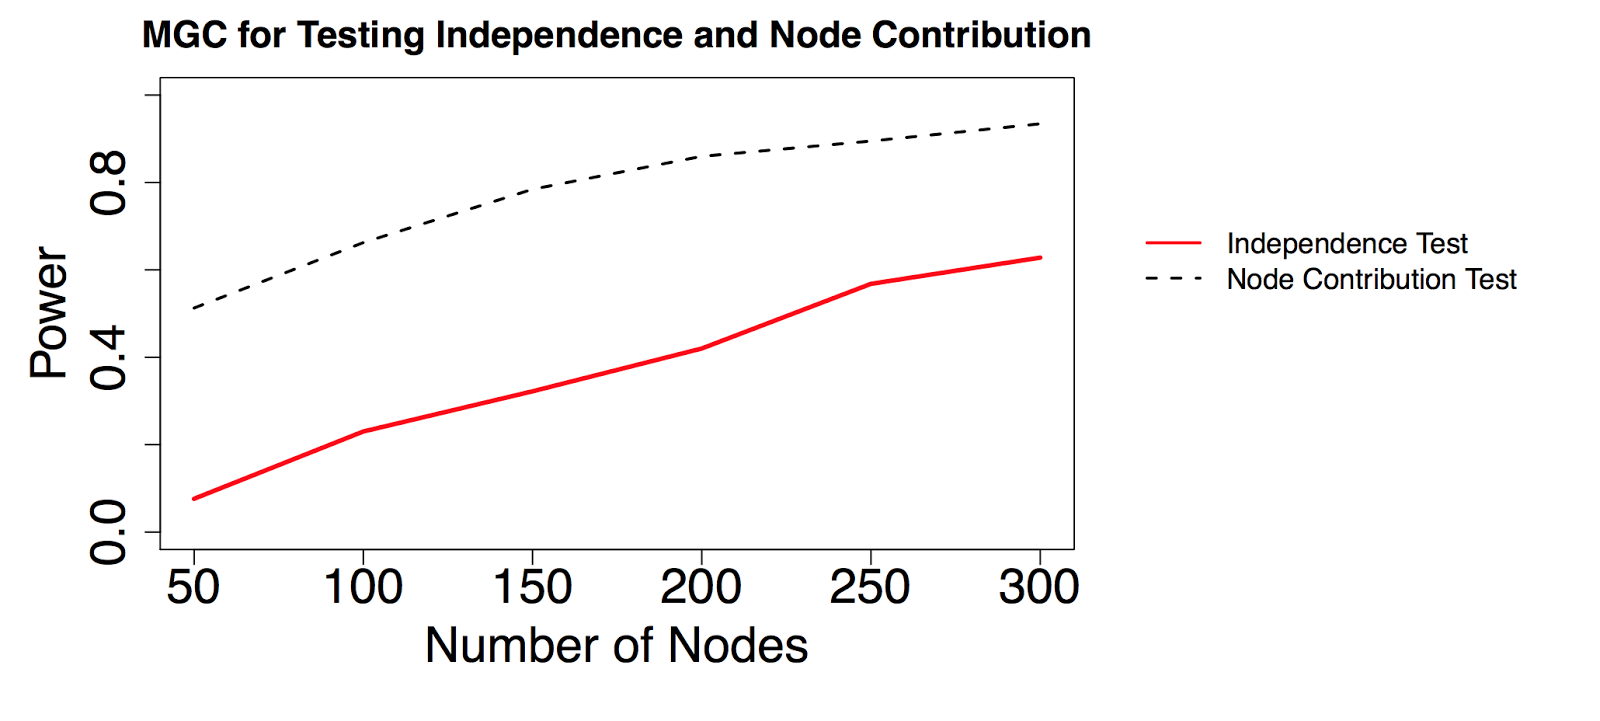
\includegraphics[width=0.95\textwidth]{../../figs/mgcPow.png}
%\caption{
%This figure considers a mixture model in the graph domain,
%where half the nodes are dependent to their attributes, and the other
%half nodes are independently generated from the attributes. We calculate
%the MGC statistic and its power for dependence testing, as well as the
%node contribution statistic and its power, i.e., the percentage of all
%dependent nodes that are ranked among the first half by $w_i$.  Indeed,
%the power plot not only shows that our node contribution algorithm can
%successfully identifies all important nodes at mildly large sample size,
%but also hints a tight relationship between $w_i$ and $C*$ that is
%worthy of further investigation. 
%}
%\label{fig:mgcP}
%\end{cframed}
%\end{figure}
%
%
%\subsection{Synaptome Statistics}
%
%We have continued to examine the Kristina15 synaptome dataset and have
%now added the Weiler Chessboard dataset to our explorations.  Using 
%\verb+meda+, and other methods along the way, we have started to compare
%the structure of these two datasets, see figure~\ref{fig:synClaw}.  
%
%\begin{figure}[h!]
%\begin{cframed}
%\centering
%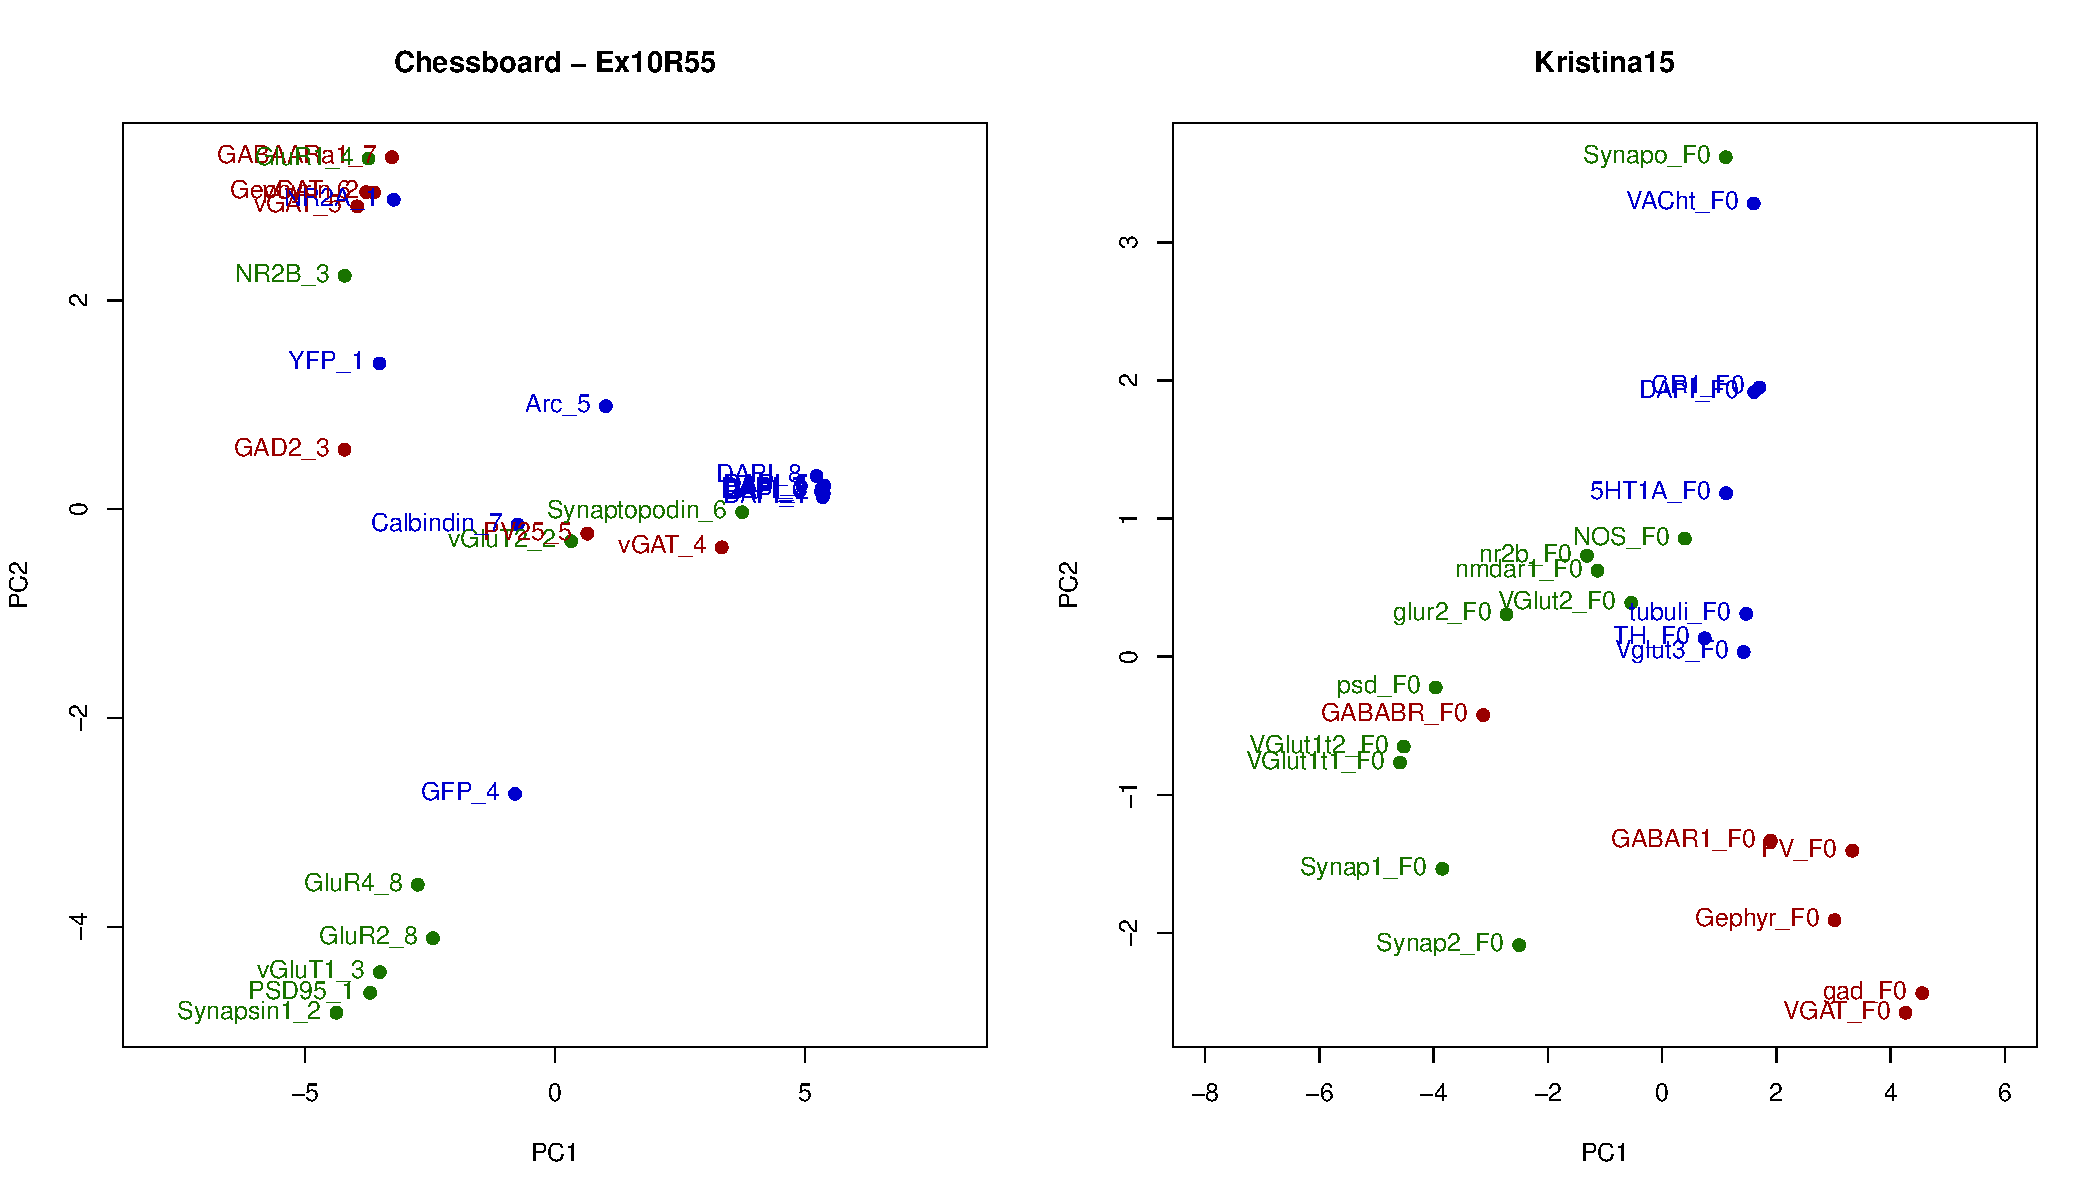
\includegraphics[width=\textwidth]{../../figs/2dProjClaw.pdf}
%\caption{
%  Principal Component Analysis (PCA) has been run on the correlation
%  matrices of both of these dataset respectively.  The first two
%  principal components are plotted against each other.  The colors
%  correspond to the type of marker, (``excitatory'' -- green,
%  ``inhibitory'' -- red, ``other'' -- blue).  Notice that some markers are
%  different between datasets, but there is a similar "claw" structure
%  present. 
%}
%\label{fig:synClaw}
%\end{cframed}
%\end{figure}

\end{document}
